\documentclass[1p]{elsarticle_modified}
%\bibliographystyle{elsarticle-num}

%\usepackage[colorlinks]{hyperref}
%\usepackage{abbrmath_seonhwa} %\Abb, \Ascr, \Acal ,\Abf, \Afrak
\usepackage{amsfonts}
\usepackage{amssymb}
\usepackage{amsmath}
\usepackage{amsthm}
\usepackage{scalefnt}
\usepackage{amsbsy}
\usepackage{kotex}
\usepackage{caption}
\usepackage{subfig}
\usepackage{color}
\usepackage{graphicx}
\usepackage{xcolor} %% white, black, red, green, blue, cyan, magenta, yellow
\usepackage{float}
\usepackage{setspace}
\usepackage{hyperref}

\usepackage{tikz}
\usetikzlibrary{arrows}

\usepackage{multirow}
\usepackage{array} % fixed length table
\usepackage{hhline}

%%%%%%%%%%%%%%%%%%%%%
\makeatletter
\renewcommand*\env@matrix[1][\arraystretch]{%
	\edef\arraystretch{#1}%
	\hskip -\arraycolsep
	\let\@ifnextchar\new@ifnextchar
	\array{*\c@MaxMatrixCols c}}
\makeatother %https://tex.stackexchange.com/questions/14071/how-can-i-increase-the-line-spacing-in-a-matrix
%%%%%%%%%%%%%%%

\usepackage[normalem]{ulem}

\newcommand{\msout}[1]{\ifmmode\text{\sout{\ensuremath{#1}}}\else\sout{#1}\fi}
%SOURCE: \msout is \stkout macro in https://tex.stackexchange.com/questions/20609/strikeout-in-math-mode

\newcommand{\cancel}[1]{
	\ifmmode
	{\color{red}\msout{#1}}
	\else
	{\color{red}\sout{#1}}
	\fi
}

\newcommand{\add}[1]{
	{\color{blue}\uwave{#1}}
}

\newcommand{\replace}[2]{
	\ifmmode
	{\color{red}\msout{#1}}{\color{blue}\uwave{#2}}
	\else
	{\color{red}\sout{#1}}{\color{blue}\uwave{#2}}
	\fi
}

\newcommand{\Sol}{\mathcal{S}} %segment
\newcommand{\D}{D} %diagram
\newcommand{\A}{\mathcal{A}} %arc


%%%%%%%%%%%%%%%%%%%%%%%%%%%%%5 test

\def\sl{\operatorname{\textup{SL}}(2,\Cbb)}
\def\psl{\operatorname{\textup{PSL}}(2,\Cbb)}
\def\quan{\mkern 1mu \triangleright \mkern 1mu}

\theoremstyle{definition}
\newtheorem{thm}{Theorem}[section]
\newtheorem{prop}[thm]{Proposition}
\newtheorem{lem}[thm]{Lemma}
\newtheorem{ques}[thm]{Question}
\newtheorem{cor}[thm]{Corollary}
\newtheorem{defn}[thm]{Definition}
\newtheorem{exam}[thm]{Example}
\newtheorem{rmk}[thm]{Remark}
\newtheorem{alg}[thm]{Algorithm}

\newcommand{\I}{\sqrt{-1}}
\begin{document}

%\begin{frontmatter}
%
%\title{Boundary parabolic representations of knots up to 8 crossings}
%
%%% Group authors per affiliation:
%\author{Yunhi Cho} 
%\address{Department of Mathematics, University of Seoul, Seoul, Korea}
%\ead{yhcho@uos.ac.kr}
%
%
%\author{Seonhwa Kim} %\fnref{s_kim}}
%\address{Center for Geometry and Physics, Institute for Basic Science, Pohang, 37673, Korea}
%\ead{ryeona17@ibs.re.kr}
%
%\author{Hyuk Kim}
%\address{Department of Mathematical Sciences, Seoul National University, Seoul 08826, Korea}
%\ead{hyukkim@snu.ac.kr}
%
%\author{Seokbeom Yoon}
%\address{Department of Mathematical Sciences, Seoul National University, Seoul, 08826,  Korea}
%\ead{sbyoon15@snu.ac.kr}
%
%\begin{abstract}
%We find all boundary parabolic representation of knots up to 8 crossings.
%
%\end{abstract}
%\begin{keyword}
%    \MSC[2010] 57M25 
%\end{keyword}
%
%\end{frontmatter}

%\linenumbers
%\tableofcontents
%
\newcommand\colored[1]{\textcolor{white}{\rule[-0.35ex]{0.8em}{1.4ex}}\kern-0.8em\color{red} #1}%
%\newcommand\colored[1]{\textcolor{white}{ #1}\kern-2.17ex	\textcolor{white}{ #1}\kern-1.81ex	\textcolor{white}{ #1}\kern-2.15ex\color{red}#1	}

{\Large $\underline{12a_{0923}~(K12a_{0923})}$}

\setlength{\tabcolsep}{10pt}
\renewcommand{\arraystretch}{1.6}
\vspace{1cm}\begin{tabular}{m{100pt}>{\centering\arraybackslash}m{274pt}}
\multirow{5}{120pt}{
	\centering
	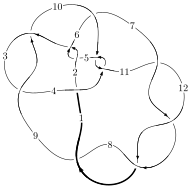
\includegraphics[width=112pt]{../../../GIT/diagram.site/Diagrams/png/1724_12a_0923.png}\\
\ \ \ A knot diagram\footnotemark}&
\allowdisplaybreaks
\textbf{Linearized knot diagam} \\
\cline{2-2}
 &
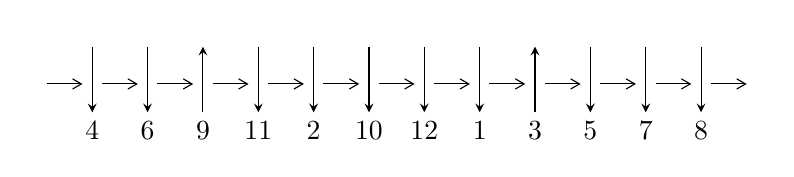
\begin{tikzpicture}[x=20pt, y=17pt]
	% nodes
	\node (C0) at (0, 0) {};
	\node (C1) at (1, 0) {};
	\node (C1U) at (1, +1) {};
	\node (C1D) at (1, -1) {4};

	\node (C2) at (2, 0) {};
	\node (C2U) at (2, +1) {};
	\node (C2D) at (2, -1) {6};

	\node (C3) at (3, 0) {};
	\node (C3U) at (3, +1) {};
	\node (C3D) at (3, -1) {9};

	\node (C4) at (4, 0) {};
	\node (C4U) at (4, +1) {};
	\node (C4D) at (4, -1) {11};

	\node (C5) at (5, 0) {};
	\node (C5U) at (5, +1) {};
	\node (C5D) at (5, -1) {2};

	\node (C6) at (6, 0) {};
	\node (C6U) at (6, +1) {};
	\node (C6D) at (6, -1) {10};

	\node (C7) at (7, 0) {};
	\node (C7U) at (7, +1) {};
	\node (C7D) at (7, -1) {12};

	\node (C8) at (8, 0) {};
	\node (C8U) at (8, +1) {};
	\node (C8D) at (8, -1) {1};

	\node (C9) at (9, 0) {};
	\node (C9U) at (9, +1) {};
	\node (C9D) at (9, -1) {3};

	\node (C10) at (10, 0) {};
	\node (C10U) at (10, +1) {};
	\node (C10D) at (10, -1) {5};

	\node (C11) at (11, 0) {};
	\node (C11U) at (11, +1) {};
	\node (C11D) at (11, -1) {7};

	\node (C12) at (12, 0) {};
	\node (C12U) at (12, +1) {};
	\node (C12D) at (12, -1) {8};
	\node (C13) at (13, 0) {};

	% arrows
	\draw[->,>={angle 60}]
	(C0) edge (C1) (C1) edge (C2) (C2) edge (C3) (C3) edge (C4) (C4) edge (C5) (C5) edge (C6) (C6) edge (C7) (C7) edge (C8) (C8) edge (C9) (C9) edge (C10) (C10) edge (C11) (C11) edge (C12) (C12) edge (C13) ;	\draw[->,>=stealth]
	(C1U) edge (C1D) (C2U) edge (C2D) (C3D) edge (C3U) (C4U) edge (C4D) (C5U) edge (C5D) (C6U) edge (C6D) (C7U) edge (C7D) (C8U) edge (C8D) (C9D) edge (C9U) (C10U) edge (C10D) (C11U) edge (C11D) (C12U) edge (C12D) ;
	\end{tikzpicture} \\
\hhline{~~} \\& 
\textbf{Solving Sequence} \\ \cline{2-2} 
 &
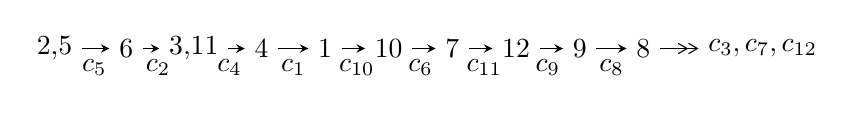
\begin{tikzpicture}[x=23pt, y=7pt]
	% node
	\node (A0) at (-1/8, 0) {2,5};
	\node (A1) at (1, 0) {6};
	\node (A2) at (33/16, 0) {3,11};
	\node (A3) at (25/8, 0) {4};
	\node (A4) at (33/8, 0) {1};
	\node (A5) at (41/8, 0) {10};
	\node (A6) at (49/8, 0) {7};
	\node (A7) at (57/8, 0) {12};
	\node (A8) at (65/8, 0) {9};
	\node (A9) at (73/8, 0) {8};
	\node (C1) at (1/2, -1) {$c_{5}$};
	\node (C2) at (3/2, -1) {$c_{2}$};
	\node (C3) at (21/8, -1) {$c_{4}$};
	\node (C4) at (29/8, -1) {$c_{1}$};
	\node (C5) at (37/8, -1) {$c_{10}$};
	\node (C6) at (45/8, -1) {$c_{6}$};
	\node (C7) at (53/8, -1) {$c_{11}$};
	\node (C8) at (61/8, -1) {$c_{9}$};
	\node (C9) at (69/8, -1) {$c_{8}$};
	\node (A10) at (11, 0) {$c_{3},c_{7},c_{12}$};

	% edge
	\draw[->,>=stealth]	
	(A0) edge (A1) (A1) edge (A2) (A2) edge (A3) (A3) edge (A4) (A4) edge (A5) (A5) edge (A6) (A6) edge (A7) (A7) edge (A8) (A8) edge (A9) ;
	\draw[->>,>={angle 60}]	
	(A9) edge (A10);
\end{tikzpicture} \\ 

\end{tabular} \\

\footnotetext{
The image of knot diagram is generated by the software ``\textbf{Draw programme}" developed by Andrew Bartholomew(\url{http://www.layer8.co.uk/maths/draw/index.htm\#Running-draw}), where we modified some parts for our purpose(\url{https://github.com/CATsTAILs/LinksPainter}).
}\phantom \\ \newline 
\centering \textbf{Ideals for irreducible components\footnotemark of $X_{\text{par}}$} 
 
\begin{align*}
I^u_{1}&=\langle 
-169316 u^{55}+765227 u^{54}+\cdots+1990656 b+207504590,\\
\phantom{I^u_{1}}&\phantom{= \langle  }64741301 u^{55}-347996846 u^{54}+\cdots+709337088 a-165503765534,\\
\phantom{I^u_{1}}&\phantom{= \langle  }u^{56}-6 u^{55}+\cdots-5065 u+2138\rangle \\
I^u_{2}&=\langle 
u^5+b+u,\;-7 u^5-2 u^4+u^3+u^2+5 a-8 u-3,\;u^6+u^4+2 u^2+1\rangle \\
I^u_{3}&=\langle 
- a^2+b- a,\;a^3+2 a^2+a-1,\;u+1\rangle \\
I^u_{4}&=\langle 
b^4 a^2-2 b^3 a+2 b^2 a^2- b^2 a+b^2-2 b a+a^2+b- a-1,\;u+1\rangle \\
\\
I^v_{1}&=\langle 
a,\;b^6+2 b^4+b^3+b^2+b-1,\;v-1\rangle \\
\end{align*}
\raggedright * 4 irreducible components of $\dim_{\mathbb{C}}=0$, with total 71 representations.\\
\raggedright * 1 irreducible components of $\dim_{\mathbb{C}}=1$ \\
\footnotetext{All coefficients of polynomials are rational numbers. But the coefficients are sometimes approximated in decimal forms when there is not enough margin.}
\newpage
\renewcommand{\arraystretch}{1}
\centering \section*{I. $I^u_{1}= \langle -1.69\times10^{5} u^{55}+7.65\times10^{5} u^{54}+\cdots+1.99\times10^{6} b+2.08\times10^{8},\;6.47\times10^{7} u^{55}-3.48\times10^{8} u^{54}+\cdots+7.09\times10^{8} a-1.66\times10^{11},\;u^{56}-6 u^{55}+\cdots-5065 u+2138 \rangle$}
\flushleft \textbf{(i) Arc colorings}\\
\begin{tabular}{m{7pt} m{180pt} m{7pt} m{180pt} }
\flushright $a_{2}=$&$\begin{pmatrix}0\\u\end{pmatrix}$ \\
\flushright $a_{5}=$&$\begin{pmatrix}1\\0\end{pmatrix}$ \\
\flushright $a_{6}=$&$\begin{pmatrix}1\\u^2\end{pmatrix}$ \\
\flushright $a_{3}=$&$\begin{pmatrix}- u\\- u^3+u\end{pmatrix}$ \\
\flushright $a_{11}=$&$\begin{pmatrix}-0.0912701 u^{55}+0.490594 u^{54}+\cdots-305.555 u+233.322\\0.0850554 u^{55}-0.384409 u^{54}+\cdots+202.825 u-104.239\end{pmatrix}$ \\
\flushright $a_{4}=$&$\begin{pmatrix}-0.0214370 u^{55}+0.107795 u^{54}+\cdots-64.6193 u+46.3327\\0.00435384 u^{55}-0.0207994 u^{54}+\cdots+12.3366 u-6.37981\end{pmatrix}$ \\
\flushright $a_{1}=$&$\begin{pmatrix}0.0281056 u^{55}-0.145026 u^{54}+\cdots+85.8717 u-67.5545\\-0.0278343 u^{55}+0.123449 u^{54}+\cdots-62.7416 u+34.1313\end{pmatrix}$ \\
\flushright $a_{10}=$&$\begin{pmatrix}-0.00621477 u^{55}+0.106185 u^{54}+\cdots-102.730 u+129.082\\0.0850554 u^{55}-0.384409 u^{54}+\cdots+202.825 u-104.239\end{pmatrix}$ \\
\flushright $a_{7}=$&$\begin{pmatrix}0.0442234 u^{55}-0.241015 u^{54}+\cdots+145.317 u-135.156\\-0.0182020 u^{55}+0.0910577 u^{54}+\cdots-54.3352 u+39.5251\end{pmatrix}$ \\
\flushright $a_{12}=$&$\begin{pmatrix}0.111606 u^{55}-0.585341 u^{54}+\cdots+348.486 u-276.321\\0.0596452 u^{55}-0.316842 u^{54}+\cdots+200.960 u-123.452\end{pmatrix}$ \\
\flushright $a_{9}=$&$\begin{pmatrix}0.0627283 u^{55}-0.266879 u^{54}+\cdots+135.607 u-49.3441\\0.0142003 u^{55}-0.0564472 u^{54}+\cdots+22.6996 u-12.6041\end{pmatrix}$ \\
\flushright $a_{8}=$&$\begin{pmatrix}0.180172 u^{55}-0.822387 u^{54}+\cdots+451.374 u-189.430\\0.0792387 u^{55}-0.456648 u^{54}+\cdots+304.815 u-239.788\end{pmatrix}$\\&\end{tabular}
\flushleft \textbf{(ii) Obstruction class $= -1$}\\~\\
\flushleft \textbf{(iii) Cusp Shapes $= -\frac{563051}{2985984} u^{55}+\frac{2308397}{2985984} u^{54}+\cdots-\frac{186951611}{497664} u+\frac{9690719}{186624}$}\\~\\
\newpage\renewcommand{\arraystretch}{1}
\flushleft \textbf{(iv) u-Polynomials at the component}\newline \\
\begin{tabular}{m{50pt}|m{274pt}}
Crossings & \hspace{64pt}u-Polynomials at each crossing \\
\hline $$\begin{aligned}c_{1}\end{aligned}$$&$\begin{aligned}
&16(16 u^{56}-48 u^{55}+\cdots+388278 u+882567)
\end{aligned}$\\
\hline $$\begin{aligned}c_{2},c_{5}\end{aligned}$$&$\begin{aligned}
&u^{56}-6 u^{55}+\cdots-5065 u+2138
\end{aligned}$\\
\hline $$\begin{aligned}c_{3},c_{9}\end{aligned}$$&$\begin{aligned}
&9(9 u^{56}-9 u^{55}+\cdots+80 u+25)
\end{aligned}$\\
\hline $$\begin{aligned}c_{4},c_{10}\end{aligned}$$&$\begin{aligned}
&9(9 u^{56}-9 u^{55}+\cdots-50 u+25)
\end{aligned}$\\
\hline $$\begin{aligned}c_{6}\end{aligned}$$&$\begin{aligned}
&16(16 u^{56}+32 u^{55}+\cdots+735282 u+119709)
\end{aligned}$\\
\hline $$\begin{aligned}c_{7},c_{8},c_{11}\\c_{12}\end{aligned}$$&$\begin{aligned}
&u^{56}+4 u^{55}+\cdots-7 u+62
\end{aligned}$\\
\hline
\end{tabular}\\~\\
\newpage\renewcommand{\arraystretch}{1}
\flushleft \textbf{(v) Riley Polynomials at the component}\newline \\
\begin{tabular}{m{50pt}|m{274pt}}
Crossings & \hspace{64pt}Riley Polynomials at each crossing \\
\hline $$\begin{aligned}c_{1}\end{aligned}$$&$\begin{aligned}
&256\\
&\cdot(256 y^{56}-11136 y^{55}+\cdots-10663154787870 y+778924509489)
\end{aligned}$\\
\hline $$\begin{aligned}c_{2},c_{5}\end{aligned}$$&$\begin{aligned}
&y^{56}-32 y^{55}+\cdots-6390845 y+4571044
\end{aligned}$\\
\hline $$\begin{aligned}c_{3},c_{9}\end{aligned}$$&$\begin{aligned}
&81(81 y^{56}+4239 y^{55}+\cdots+12400 y+625)
\end{aligned}$\\
\hline $$\begin{aligned}c_{4},c_{10}\end{aligned}$$&$\begin{aligned}
&81(81 y^{56}+1971 y^{55}+\cdots+16400 y+625)
\end{aligned}$\\
\hline $$\begin{aligned}c_{6}\end{aligned}$$&$\begin{aligned}
&256(256 y^{56}-10624 y^{55}+\cdots-1.77562\times10^{11} y+1.43302\times10^{10})
\end{aligned}$\\
\hline $$\begin{aligned}c_{7},c_{8},c_{11}\\c_{12}\end{aligned}$$&$\begin{aligned}
&y^{56}-66 y^{55}+\cdots-2901 y+3844
\end{aligned}$\\
\hline
\end{tabular}\\~\\
\newpage\flushleft \textbf{(vi) Complex Volumes and Cusp Shapes}
$$\begin{array}{c|c|c}  
\text{Solutions to }I^u_{1}& \I (\text{vol} + \sqrt{-1}CS) & \text{Cusp shape}\\
 \hline 
\begin{aligned}
u &= \phantom{-}0.984706 + 0.213928 I \\
a &= \phantom{-}2.54376 - 1.38909 I \\
b &= \phantom{-}0.219398 + 0.692771 I\end{aligned}
 & -10.33120 - 0.88863 I & -11.9568 + 8.3028 I \\ \hline\begin{aligned}
u &= \phantom{-}0.984706 - 0.213928 I \\
a &= \phantom{-}2.54376 + 1.38909 I \\
b &= \phantom{-}0.219398 - 0.692771 I\end{aligned}
 & -10.33120 + 0.88863 I & -11.9568 - 8.3028 I \\ \hline\begin{aligned}
u &= \phantom{-}0.981741 + 0.367067 I \\
a &= -1.39029 + 1.32174 I \\
b &= -0.297204 - 0.885770 I\end{aligned}
 & -1.84811 - 1.66866 I & -10.40782 + 3.06587 I \\ \hline\begin{aligned}
u &= \phantom{-}0.981741 - 0.367067 I \\
a &= -1.39029 - 1.32174 I \\
b &= -0.297204 + 0.885770 I\end{aligned}
 & -1.84811 + 1.66866 I & -10.40782 - 3.06587 I \\ \hline\begin{aligned}
u &= -0.392152 + 0.823059 I \\
a &= \phantom{-}0.331863 + 0.870571 I \\
b &= -0.459949 - 0.211030 I\end{aligned}
 & -4.33948 + 2.58823 I & -15.9377 - 3.4312 I \\ \hline\begin{aligned}
u &= -0.392152 - 0.823059 I \\
a &= \phantom{-}0.331863 - 0.870571 I \\
b &= -0.459949 + 0.211030 I\end{aligned}
 & -4.33948 - 2.58823 I & -15.9377 + 3.4312 I \\ \hline\begin{aligned}
u &= -0.210486 + 0.885885 I \\
a &= -0.754309 - 0.859129 I \\
b &= \phantom{-}0.916464 + 0.273165 I\end{aligned}
 & -13.7069 + 4.2294 I & -15.0908 - 2.2409 I \\ \hline\begin{aligned}
u &= -0.210486 - 0.885885 I \\
a &= -0.754309 + 0.859129 I \\
b &= \phantom{-}0.916464 - 0.273165 I\end{aligned}
 & -13.7069 - 4.2294 I & -15.0908 + 2.2409 I \\ \hline\begin{aligned}
u &= -1.117840 + 0.121937 I \\
a &= \phantom{-}0.183222 - 0.754249 I \\
b &= -0.175598 - 0.720988 I\end{aligned}
 & -2.33703 - 0.81235 I & -9.18182 + 8.94342 I \\ \hline\begin{aligned}
u &= -1.117840 - 0.121937 I \\
a &= \phantom{-}0.183222 + 0.754249 I \\
b &= -0.175598 + 0.720988 I\end{aligned}
 & -2.33703 + 0.81235 I & -9.18182 - 8.94342 I\\
 \hline 
 \end{array}$$\newpage$$\begin{array}{c|c|c}  
\text{Solutions to }I^u_{1}& \I (\text{vol} + \sqrt{-1}CS) & \text{Cusp shape}\\
 \hline 
\begin{aligned}
u &= \phantom{-}0.783032 + 0.807710 I \\
a &= -0.52560 + 1.38392 I \\
b &= -0.010851 - 1.124970 I\end{aligned}
 & -1.59922 - 2.81223 I & -5.39241 + 2.86664 I \\ \hline\begin{aligned}
u &= \phantom{-}0.783032 - 0.807710 I \\
a &= -0.52560 - 1.38392 I \\
b &= -0.010851 + 1.124970 I\end{aligned}
 & -1.59922 + 2.81223 I & -5.39241 - 2.86664 I \\ \hline\begin{aligned}
u &= -0.066075 + 1.135000 I \\
a &= -0.36094 - 1.62838 I \\
b &= \phantom{-}0.615579 + 1.197570 I\end{aligned}
 & -10.9441 - 9.8213 I & -12.63911 + 5.52696 I \\ \hline\begin{aligned}
u &= -0.066075 - 1.135000 I \\
a &= -0.36094 + 1.62838 I \\
b &= \phantom{-}0.615579 - 1.197570 I\end{aligned}
 & -10.9441 + 9.8213 I & -12.63911 - 5.52696 I \\ \hline\begin{aligned}
u &= \phantom{-}0.411231 + 0.747950 I \\
a &= \phantom{-}0.36943 - 1.47797 I \\
b &= -0.166040 + 1.104020 I\end{aligned}
 & \phantom{-}3.36428 - 0.23401 I & -0.97991 + 2.43933 I \\ \hline\begin{aligned}
u &= \phantom{-}0.411231 - 0.747950 I \\
a &= \phantom{-}0.36943 + 1.47797 I \\
b &= -0.166040 - 1.104020 I\end{aligned}
 & \phantom{-}3.36428 + 0.23401 I & -0.97991 - 2.43933 I \\ \hline\begin{aligned}
u &= \phantom{-}1.098780 + 0.455875 I \\
a &= \phantom{-}1.02438 - 1.04747 I \\
b &= \phantom{-}0.490597 + 1.118040 I\end{aligned}
 & \phantom{-}1.18518 - 4.32062 I & -5.36534 + 4.17876 I \\ \hline\begin{aligned}
u &= \phantom{-}1.098780 - 0.455875 I \\
a &= \phantom{-}1.02438 + 1.04747 I \\
b &= \phantom{-}0.490597 - 1.118040 I\end{aligned}
 & \phantom{-}1.18518 + 4.32062 I & -5.36534 - 4.17876 I \\ \hline\begin{aligned}
u &= -1.182510 + 0.227112 I \\
a &= -0.429835 + 0.746826 I \\
b &= \phantom{-}0.377689 + 0.830409 I\end{aligned}
 & -9.97809 - 1.88428 I & -12.95942 + 3.16374 I \\ \hline\begin{aligned}
u &= -1.182510 - 0.227112 I \\
a &= -0.429835 - 0.746826 I \\
b &= \phantom{-}0.377689 - 0.830409 I\end{aligned}
 & -9.97809 + 1.88428 I & -12.95942 - 3.16374 I\\
 \hline 
 \end{array}$$\newpage$$\begin{array}{c|c|c}  
\text{Solutions to }I^u_{1}& \I (\text{vol} + \sqrt{-1}CS) & \text{Cusp shape}\\
 \hline 
\begin{aligned}
u &= -0.651226 + 1.017980 I \\
a &= \phantom{-}0.229212 + 1.095150 I \\
b &= -0.154199 - 0.511987 I\end{aligned}
 & -4.36511 + 2.70896 I & -17.8835 - 1.9240 I \\ \hline\begin{aligned}
u &= -0.651226 - 1.017980 I \\
a &= \phantom{-}0.229212 - 1.095150 I \\
b &= -0.154199 + 0.511987 I\end{aligned}
 & -4.36511 - 2.70896 I & -17.8835 + 1.9240 I \\ \hline\begin{aligned}
u &= -0.118014 + 1.203290 I \\
a &= \phantom{-}0.30642 + 1.47527 I \\
b &= -0.503344 - 1.061300 I\end{aligned}
 & -2.28016 - 6.66641 I & -11.44494 + 7.11180 I \\ \hline\begin{aligned}
u &= -0.118014 - 1.203290 I \\
a &= \phantom{-}0.30642 - 1.47527 I \\
b &= -0.503344 + 1.061300 I\end{aligned}
 & -2.28016 + 6.66641 I & -11.44494 - 7.11180 I \\ \hline\begin{aligned}
u &= \phantom{-}0.143056 + 0.772743 I \\
a &= \phantom{-}0.641494 - 1.196870 I \\
b &= -0.574548 + 1.166620 I\end{aligned}
 & -5.75586 + 5.22238 I & -8.67240 - 3.67476 I \\ \hline\begin{aligned}
u &= \phantom{-}0.143056 - 0.772743 I \\
a &= \phantom{-}0.641494 + 1.196870 I \\
b &= -0.574548 - 1.166620 I\end{aligned}
 & -5.75586 - 5.22238 I & -8.67240 + 3.67476 I \\ \hline\begin{aligned}
u &= \phantom{-}0.233014 + 0.741341 I \\
a &= -0.428118 + 1.316410 I \\
b &= \phantom{-}0.373389 - 1.116040 I\end{aligned}
 & \phantom{-}2.07162 + 3.27052 I & -5.16362 - 5.02421 I \\ \hline\begin{aligned}
u &= \phantom{-}0.233014 - 0.741341 I \\
a &= -0.428118 - 1.316410 I \\
b &= \phantom{-}0.373389 + 1.116040 I\end{aligned}
 & \phantom{-}2.07162 - 3.27052 I & -5.16362 + 5.02421 I \\ \hline\begin{aligned}
u &= \phantom{-}1.154880 + 0.445094 I \\
a &= -0.940220 + 0.970110 I \\
b &= -0.705436 - 1.185240 I\end{aligned}
 & -0.73558 - 7.71938 I & -8.00000 + 9.01590 I \\ \hline\begin{aligned}
u &= \phantom{-}1.154880 - 0.445094 I \\
a &= -0.940220 - 0.970110 I \\
b &= -0.705436 + 1.185240 I\end{aligned}
 & -0.73558 + 7.71938 I & -8.00000 - 9.01590 I\\
 \hline 
 \end{array}$$\newpage$$\begin{array}{c|c|c}  
\text{Solutions to }I^u_{1}& \I (\text{vol} + \sqrt{-1}CS) & \text{Cusp shape}\\
 \hline 
\begin{aligned}
u &= \phantom{-}1.186190 + 0.441930 I \\
a &= \phantom{-}0.863048 - 0.971863 I \\
b &= \phantom{-}0.89596 + 1.24873 I\end{aligned}
 & -8.91014 - 9.70074 I & \phantom{-0.000000 } 0 \\ \hline\begin{aligned}
u &= \phantom{-}1.186190 - 0.441930 I \\
a &= \phantom{-}0.863048 + 0.971863 I \\
b &= \phantom{-}0.89596 - 1.24873 I\end{aligned}
 & -8.91014 + 9.70074 I & \phantom{-0.000000 } 0 \\ \hline\begin{aligned}
u &= -0.281565 + 1.254220 I \\
a &= -0.289928 - 1.294920 I \\
b &= \phantom{-}0.396705 + 0.868356 I\end{aligned}
 & -0.09114 - 1.67831 I & \phantom{-0.000000 } 0 \\ \hline\begin{aligned}
u &= -0.281565 - 1.254220 I \\
a &= -0.289928 + 1.294920 I \\
b &= \phantom{-}0.396705 - 0.868356 I\end{aligned}
 & -0.09114 + 1.67831 I & \phantom{-0.000000 } 0 \\ \hline\begin{aligned}
u &= \phantom{-}1.324820 + 0.384063 I \\
a &= \phantom{-}0.055551 + 0.278282 I \\
b &= -1.364170 + 0.268279 I\end{aligned}
 & -18.4368 - 8.6427 I & \phantom{-0.000000 } 0 \\ \hline\begin{aligned}
u &= \phantom{-}1.324820 - 0.384063 I \\
a &= \phantom{-}0.055551 - 0.278282 I \\
b &= -1.364170 - 0.268279 I\end{aligned}
 & -18.4368 + 8.6427 I & \phantom{-0.000000 } 0 \\ \hline\begin{aligned}
u &= \phantom{-}1.335470 + 0.358449 I \\
a &= \phantom{-}0.0527808 - 0.1215550 I \\
b &= \phantom{-}1.127220 - 0.238919 I\end{aligned}
 & -9.45136 - 6.69405 I & \phantom{-0.000000 } 0 \\ \hline\begin{aligned}
u &= \phantom{-}1.335470 - 0.358449 I \\
a &= \phantom{-}0.0527808 + 0.1215550 I \\
b &= \phantom{-}1.127220 + 0.238919 I\end{aligned}
 & -9.45136 + 6.69405 I & \phantom{-0.000000 } 0 \\ \hline\begin{aligned}
u &= -1.225400 + 0.652300 I \\
a &= -0.32305 - 1.43167 I \\
b &= -0.732798 + 0.721623 I\end{aligned}
 & -16.5150 + 1.3611 I & \phantom{-0.000000 } 0 \\ \hline\begin{aligned}
u &= -1.225400 - 0.652300 I \\
a &= -0.32305 + 1.43167 I \\
b &= -0.732798 - 0.721623 I\end{aligned}
 & -16.5150 - 1.3611 I & \phantom{-0.000000 } 0\\
 \hline 
 \end{array}$$\newpage$$\begin{array}{c|c|c}  
\text{Solutions to }I^u_{1}& \I (\text{vol} + \sqrt{-1}CS) & \text{Cusp shape}\\
 \hline 
\begin{aligned}
u &= \phantom{-}1.37863 + 0.31544 I \\
a &= -0.092380 - 0.165122 I \\
b &= -0.799954 + 0.318153 I\end{aligned}
 & -6.21382 - 3.21160 I & \phantom{-0.000000 } 0 \\ \hline\begin{aligned}
u &= \phantom{-}1.37863 - 0.31544 I \\
a &= -0.092380 + 0.165122 I \\
b &= -0.799954 - 0.318153 I\end{aligned}
 & -6.21382 + 3.21160 I & \phantom{-0.000000 } 0 \\ \hline\begin{aligned}
u &= -1.35351 + 0.56530 I \\
a &= -0.87548 - 1.35090 I \\
b &= -0.72269 + 1.34990 I\end{aligned}
 & -15.0022 + 15.8154 I & \phantom{-0.000000 } 0 \\ \hline\begin{aligned}
u &= -1.35351 - 0.56530 I \\
a &= -0.87548 + 1.35090 I \\
b &= -0.72269 - 1.34990 I\end{aligned}
 & -15.0022 - 15.8154 I & \phantom{-0.000000 } 0 \\ \hline\begin{aligned}
u &= -1.36457 + 0.58672 I \\
a &= \phantom{-}0.77901 + 1.28814 I \\
b &= \phantom{-}0.65208 - 1.26539 I\end{aligned}
 & -6.2885 + 12.9423 I & \phantom{-0.000000 } 0 \\ \hline\begin{aligned}
u &= -1.36457 - 0.58672 I \\
a &= \phantom{-}0.77901 - 1.28814 I \\
b &= \phantom{-}0.65208 + 1.26539 I\end{aligned}
 & -6.2885 - 12.9423 I & \phantom{-0.000000 } 0 \\ \hline\begin{aligned}
u &= -1.32133 + 0.68751 I \\
a &= \phantom{-}0.471952 + 1.284130 I \\
b &= \phantom{-}0.577036 - 0.948979 I\end{aligned}
 & -6.95153 + 3.85491 I & \phantom{-0.000000 } 0 \\ \hline\begin{aligned}
u &= -1.32133 - 0.68751 I \\
a &= \phantom{-}0.471952 - 1.284130 I \\
b &= \phantom{-}0.577036 + 0.948979 I\end{aligned}
 & -6.95153 - 3.85491 I & \phantom{-0.000000 } 0 \\ \hline\begin{aligned}
u &= \phantom{-}1.46368 + 0.35591 I \\
a &= -0.123992 + 0.336867 I \\
b &= \phantom{-}0.659559 - 0.634367 I\end{aligned}
 & -7.88342 + 0.96412 I & \phantom{-0.000000 } 0 \\ \hline\begin{aligned}
u &= \phantom{-}1.46368 - 0.35591 I \\
a &= -0.123992 - 0.336867 I \\
b &= \phantom{-}0.659559 + 0.634367 I\end{aligned}
 & -7.88342 - 0.96412 I & \phantom{-0.000000 } 0\\
 \hline 
 \end{array}$$\newpage$$\begin{array}{c|c|c}  
\text{Solutions to }I^u_{1}& \I (\text{vol} + \sqrt{-1}CS) & \text{Cusp shape}\\
 \hline 
\begin{aligned}
u &= -1.37201 + 0.62798 I \\
a &= -0.645034 - 1.241570 I \\
b &= -0.581916 + 1.144830 I\end{aligned}
 & -3.77550 + 8.37956 I & \phantom{-0.000000 } 0 \\ \hline\begin{aligned}
u &= -1.37201 - 0.62798 I \\
a &= -0.645034 + 1.241570 I \\
b &= -0.581916 - 1.144830 I\end{aligned}
 & -3.77550 - 8.37956 I & \phantom{-0.000000 } 0 \\ \hline\begin{aligned}
u &= \phantom{-}1.46550 + 0.44360 I \\
a &= \phantom{-}0.324608 - 0.372587 I \\
b &= -0.689131 + 0.909581 I\end{aligned}
 & -15.9597 + 4.0146 I & \phantom{-0.000000 } 0 \\ \hline\begin{aligned}
u &= \phantom{-}1.46550 - 0.44360 I \\
a &= \phantom{-}0.324608 + 0.372587 I \\
b &= -0.689131 - 0.909581 I\end{aligned}
 & -15.9597 - 4.0146 I & \phantom{-0.000000 } 0 \\ \hline\begin{aligned}
u &= -0.288024 + 0.269790 I \\
a &= \phantom{-}0.642999 - 0.968459 I \\
b &= \phantom{-}0.136152 - 0.381527 I\end{aligned}
 & -0.573993 + 0.867939 I & -10.17045 - 7.71087 I \\ \hline\begin{aligned}
u &= -0.288024 - 0.269790 I \\
a &= \phantom{-}0.642999 + 0.968459 I \\
b &= \phantom{-}0.136152 + 0.381527 I\end{aligned}
 & -0.573993 - 0.867939 I & -10.17045 + 7.71087 I\\
 \hline 
 \end{array}$$\newpage\newpage\renewcommand{\arraystretch}{1}
\centering \section*{II. $I^u_{2}= \langle u^5+b+u,\;-7 u^5-2 u^4+u^3+u^2+5 a-8 u-3,\;u^6+u^4+2 u^2+1 \rangle$}
\flushleft \textbf{(i) Arc colorings}\\
\begin{tabular}{m{7pt} m{180pt} m{7pt} m{180pt} }
\flushright $a_{2}=$&$\begin{pmatrix}0\\u\end{pmatrix}$ \\
\flushright $a_{5}=$&$\begin{pmatrix}1\\0\end{pmatrix}$ \\
\flushright $a_{6}=$&$\begin{pmatrix}1\\u^2\end{pmatrix}$ \\
\flushright $a_{3}=$&$\begin{pmatrix}- u\\- u^3+u\end{pmatrix}$ \\
\flushright $a_{11}=$&$\begin{pmatrix}\frac{7}{5} u^5+\frac{2}{5} u^4+\cdots+\frac{8}{5} u+\frac{3}{5}\\- u^5- u\end{pmatrix}$ \\
\flushright $a_{4}=$&$\begin{pmatrix}\frac{4}{5} u^5-\frac{1}{5} u^4+\cdots+\frac{6}{5} u-\frac{4}{5}\\1\end{pmatrix}$ \\
\flushright $a_{1}=$&$\begin{pmatrix}-0.240000 u^{5}+0.560000 u^{4}+\cdots-0.160000 u+1.04000\\-\frac{1}{5} u^5-\frac{1}{5} u^4+\cdots+\frac{1}{5} u-\frac{4}{5}\end{pmatrix}$ \\
\flushright $a_{10}=$&$\begin{pmatrix}\frac{2}{5} u^5+\frac{2}{5} u^4+\cdots+\frac{3}{5} u+\frac{3}{5}\\- u^5- u\end{pmatrix}$ \\
\flushright $a_{7}=$&$\begin{pmatrix}-0.240000 u^{5}+0.560000 u^{4}+\cdots-0.160000 u+2.04000\\-\frac{1}{5} u^5-\frac{1}{5} u^4+\cdots-\frac{4}{5} u-\frac{4}{5}\end{pmatrix}$ \\
\flushright $a_{12}=$&$\begin{pmatrix}-0.0800000 u^{5}+0.520000 u^{4}+\cdots+0.280000 u+0.680000\\-\frac{2}{5} u^5-\frac{2}{5} u^4+\cdots+\frac{2}{5} u-\frac{3}{5}\end{pmatrix}$ \\
\flushright $a_{9}=$&$\begin{pmatrix}\frac{2}{5} u^5+\frac{7}{5} u^4+\cdots+\frac{3}{5} u+\frac{8}{5}\\- u^5- u^4-2 u^2- u-2\end{pmatrix}$ \\
\flushright $a_{8}=$&$\begin{pmatrix}-0.0800000 u^{5}+1.52000 u^{4}+\cdots+0.280000 u+1.68000\\-\frac{2}{5} u^5-\frac{7}{5} u^4+\cdots-\frac{3}{5} u-\frac{8}{5}\end{pmatrix}$\\&\end{tabular}
\flushleft \textbf{(ii) Obstruction class $= 1$}\\~\\
\flushleft \textbf{(iii) Cusp Shapes $= 4 u^4+4 u^2-4$}\\~\\
\newpage\renewcommand{\arraystretch}{1}
\flushleft \textbf{(iv) u-Polynomials at the component}\newline \\
\begin{tabular}{m{50pt}|m{274pt}}
Crossings & \hspace{64pt}u-Polynomials at each crossing \\
\hline $$\begin{aligned}c_{1}\end{aligned}$$&$\begin{aligned}
&5(5 u^6-14 u^5+23 u^4-24 u^3+16 u^2-6 u+1)
\end{aligned}$\\
\hline $$\begin{aligned}c_{2},c_{5}\end{aligned}$$&$\begin{aligned}
&u^6+u^4+2 u^2+1
\end{aligned}$\\
\hline $$\begin{aligned}c_{3},c_{4},c_{9}\\c_{10}\end{aligned}$$&$\begin{aligned}
&(u^2+1)^3
\end{aligned}$\\
\hline $$\begin{aligned}c_{6}\end{aligned}$$&$\begin{aligned}
&5(5 u^6+8 u^5+3 u^4+2 u^3+4 u^2+2 u+1)
\end{aligned}$\\
\hline $$\begin{aligned}c_{7},c_{8},c_{11}\\c_{12}\end{aligned}$$&$\begin{aligned}
&u^6-3 u^4+2 u^2+1
\end{aligned}$\\
\hline
\end{tabular}\\~\\
\newpage\renewcommand{\arraystretch}{1}
\flushleft \textbf{(v) Riley Polynomials at the component}\newline \\
\begin{tabular}{m{50pt}|m{274pt}}
Crossings & \hspace{64pt}Riley Polynomials at each crossing \\
\hline $$\begin{aligned}c_{1}\end{aligned}$$&$\begin{aligned}
&25(25 y^6+34 y^5+17 y^4+2 y^3+14 y^2-4 y+1)
\end{aligned}$\\
\hline $$\begin{aligned}c_{2},c_{5}\end{aligned}$$&$\begin{aligned}
&(y^3+y^2+2 y+1)^2
\end{aligned}$\\
\hline $$\begin{aligned}c_{3},c_{4},c_{9}\\c_{10}\end{aligned}$$&$\begin{aligned}
&(y+1)^6
\end{aligned}$\\
\hline $$\begin{aligned}c_{6}\end{aligned}$$&$\begin{aligned}
&25(25 y^6-34 y^5+17 y^4-2 y^3+14 y^2+4 y+1)
\end{aligned}$\\
\hline $$\begin{aligned}c_{7},c_{8},c_{11}\\c_{12}\end{aligned}$$&$\begin{aligned}
&(y^3-3 y^2+2 y+1)^2
\end{aligned}$\\
\hline
\end{tabular}\\~\\
\newpage\flushleft \textbf{(vi) Complex Volumes and Cusp Shapes}
$$\begin{array}{c|c|c}  
\text{Solutions to }I^u_{2}& \I (\text{vol} + \sqrt{-1}CS) & \text{Cusp shape}\\
 \hline 
\begin{aligned}
u &= \phantom{-}0.744862 + 0.877439 I \\
a &= \phantom{-}0.38847 - 1.86784 I \\
b &= \phantom{-0.000000 -}1.000000 I\end{aligned}
 & -3.02413 + 2.82812 I & -11.50976 + 2.97945 I \\ \hline\begin{aligned}
u &= \phantom{-}0.744862 - 0.877439 I \\
a &= \phantom{-}0.38847 + 1.86784 I \\
b &= \phantom{-0.000000 } -1.000000 I\end{aligned}
 & -3.02413 - 2.82812 I & -11.50976 - 2.97945 I \\ \hline\begin{aligned}
u &= -0.744862 + 0.877439 I \\
a &= -0.432328 - 0.895156 I \\
b &= \phantom{-0.000000 -}1.000000 I\end{aligned}
 & -3.02413 - 2.82812 I & -11.50976 - 2.97945 I \\ \hline\begin{aligned}
u &= -0.744862 - 0.877439 I \\
a &= -0.432328 + 0.895156 I \\
b &= \phantom{-0.000000 } -1.000000 I\end{aligned}
 & -3.02413 + 2.82812 I & -11.50976 + 2.97945 I \\ \hline\begin{aligned}
u &= \phantom{-0.000000 -}0.754878 I \\
a &= \phantom{-}0.84386 + 1.63701 I \\
b &= \phantom{-0.000000 } -1.000000 I\end{aligned}
 & \phantom{-}1.11345\phantom{ +0.000000I} & -4.98050\phantom{ +0.000000I} \\ \hline\begin{aligned}
u &= \phantom{-0.000000 } -0.754878 I \\
a &= \phantom{-}0.84386 - 1.63701 I \\
b &= \phantom{-0.000000 -}1.000000 I\end{aligned}
 & \phantom{-}1.11345\phantom{ +0.000000I} & -4.98050\phantom{ +0.000000I}\\
 \hline 
 \end{array}$$\newpage\newpage\renewcommand{\arraystretch}{1}
\centering \section*{III. $I^u_{3}= \langle - a^2+b- a,\;a^3+2 a^2+a-1,\;u+1 \rangle$}
\flushleft \textbf{(i) Arc colorings}\\
\begin{tabular}{m{7pt} m{180pt} m{7pt} m{180pt} }
\flushright $a_{2}=$&$\begin{pmatrix}0\\-1\end{pmatrix}$ \\
\flushright $a_{5}=$&$\begin{pmatrix}1\\0\end{pmatrix}$ \\
\flushright $a_{6}=$&$\begin{pmatrix}1\\1\end{pmatrix}$ \\
\flushright $a_{3}=$&$\begin{pmatrix}1\\0\end{pmatrix}$ \\
\flushright $a_{11}=$&$\begin{pmatrix}a\\a^2+a\end{pmatrix}$ \\
\flushright $a_{4}=$&$\begin{pmatrix}a^2+a\\- a\end{pmatrix}$ \\
\flushright $a_{1}=$&$\begin{pmatrix}- a\\- a^2- a\end{pmatrix}$ \\
\flushright $a_{10}=$&$\begin{pmatrix}a^2+2 a\\a^2+a\end{pmatrix}$ \\
\flushright $a_{7}=$&$\begin{pmatrix}a\\a^2+a\end{pmatrix}$ \\
\flushright $a_{12}=$&$\begin{pmatrix}a\\a^2+a\end{pmatrix}$ \\
\flushright $a_{9}=$&$\begin{pmatrix}a\\a^2+a\end{pmatrix}$ \\
\flushright $a_{8}=$&$\begin{pmatrix}a\\a^2+a\end{pmatrix}$\\&\end{tabular}
\flushleft \textbf{(ii) Obstruction class $= -1$}\\~\\
\flushleft \textbf{(iii) Cusp Shapes $= -6$}\\~\\
\newpage\renewcommand{\arraystretch}{1}
\flushleft \textbf{(iv) u-Polynomials at the component}\newline \\
\begin{tabular}{m{50pt}|m{274pt}}
Crossings & \hspace{64pt}u-Polynomials at each crossing \\
\hline $$\begin{aligned}c_{1},c_{3},c_{4}\\c_{9},c_{10}\end{aligned}$$&$\begin{aligned}
&u^3+u+1
\end{aligned}$\\
\hline $$\begin{aligned}c_{2},c_{5}\end{aligned}$$&$\begin{aligned}
&(u+1)^3
\end{aligned}$\\
\hline $$\begin{aligned}c_{6}\end{aligned}$$&$\begin{aligned}
&u^3+2 u^2+u-1
\end{aligned}$\\
\hline $$\begin{aligned}c_{7},c_{8},c_{11}\\c_{12}\end{aligned}$$&$\begin{aligned}
&u^3
\end{aligned}$\\
\hline
\end{tabular}\\~\\
\newpage\renewcommand{\arraystretch}{1}
\flushleft \textbf{(v) Riley Polynomials at the component}\newline \\
\begin{tabular}{m{50pt}|m{274pt}}
Crossings & \hspace{64pt}Riley Polynomials at each crossing \\
\hline $$\begin{aligned}c_{1},c_{3},c_{4}\\c_{9},c_{10}\end{aligned}$$&$\begin{aligned}
&y^3+2 y^2+y-1
\end{aligned}$\\
\hline $$\begin{aligned}c_{2},c_{5}\end{aligned}$$&$\begin{aligned}
&(y-1)^3
\end{aligned}$\\
\hline $$\begin{aligned}c_{6}\end{aligned}$$&$\begin{aligned}
&y^3-2 y^2+5 y-1
\end{aligned}$\\
\hline $$\begin{aligned}c_{7},c_{8},c_{11}\\c_{12}\end{aligned}$$&$\begin{aligned}
&y^3
\end{aligned}$\\
\hline
\end{tabular}\\~\\
\newpage\flushleft \textbf{(vi) Complex Volumes and Cusp Shapes}
$$\begin{array}{c|c|c}  
\text{Solutions to }I^u_{3}& \I (\text{vol} + \sqrt{-1}CS) & \text{Cusp shape}\\
 \hline 
\begin{aligned}
u &= -1.00000\phantom{ +0.000000I} \\
a &= -1.23279 + 0.79255 I \\
b &= -0.341164 - 1.161540 I\end{aligned}
 & -1.64493\phantom{ +0.000000I} & -6.00000\phantom{ +0.000000I} \\ \hline\begin{aligned}
u &= -1.00000\phantom{ +0.000000I} \\
a &= -1.23279 - 0.79255 I \\
b &= -0.341164 + 1.161540 I\end{aligned}
 & -1.64493\phantom{ +0.000000I} & -6.00000\phantom{ +0.000000I} \\ \hline\begin{aligned}
u &= -1.00000\phantom{ +0.000000I} \\
a &= \phantom{-}0.465571\phantom{ +0.000000I} \\
b &= \phantom{-}0.682328\phantom{ +0.000000I}\end{aligned}
 & -1.64493\phantom{ +0.000000I} & -6.00000\phantom{ +0.000000I}\\
 \hline 
 \end{array}$$\newpage\newpage\renewcommand{\arraystretch}{1}
\centering \section*{IV. $I^u_{4}= \langle b^4 a^2-2 b^3 a+2 b^2 a^2- b^2 a+b^2-2 b a+a^2+b- a-1,\;u+1 \rangle$}
\flushleft \textbf{(i) Arc colorings}\\
\begin{tabular}{m{7pt} m{180pt} m{7pt} m{180pt} }
\flushright $a_{2}=$&$\begin{pmatrix}0\\-1\end{pmatrix}$ \\
\flushright $a_{5}=$&$\begin{pmatrix}1\\0\end{pmatrix}$ \\
\flushright $a_{6}=$&$\begin{pmatrix}1\\1\end{pmatrix}$ \\
\flushright $a_{3}=$&$\begin{pmatrix}1\\0\end{pmatrix}$ \\
\flushright $a_{11}=$&$\begin{pmatrix}a\\b\end{pmatrix}$ \\
\flushright $a_{4}=$&$\begin{pmatrix}- b a+1\\- b^2\end{pmatrix}$ \\
\flushright $a_{1}=$&$\begin{pmatrix}- b^2 a^2+2 b a-1\\- b^3 a+b^2-1\end{pmatrix}$ \\
\flushright $a_{10}=$&$\begin{pmatrix}b+a\\b\end{pmatrix}$ \\
\flushright $a_{7}=$&$\begin{pmatrix}- b a- a^2+1\\- b a+1\end{pmatrix}$ \\
\flushright $a_{12}=$&$\begin{pmatrix}- b^3 a^2- a^3 b^2+2 b^2 a- a^3- b+2 a\\- b^3 a^2+2 b^2 a- a^2 b+a\end{pmatrix}$ \\
\flushright $a_{9}=$&$\begin{pmatrix}a\\b\end{pmatrix}$ \\
\flushright $a_{8}=$&$\begin{pmatrix}b^3 a^2+a^3 b^2- b^2 a^2-2 b^2 a+a^3+b a- a^2+b- a\\b^3 a^2- b^3 a-2 b^2 a+a^2 b+b^2- b a+b- a\end{pmatrix}$\\&\end{tabular}
\flushleft \textbf{(ii) Obstruction class $= 1$}\\~\\
\flushleft \textbf{(iii) Cusp Shapes $= -16$}\\~\\
\flushleft \textbf{(iv) u-Polynomials at the component} : It cannot be defined for a positive dimension component.\\~\\
\flushleft \textbf{(v) Riley Polynomials at the component} : It cannot be defined for a positive dimension component.\\~\\
\newpage\flushleft \textbf{(iv) Complex Volumes and Cusp Shapes}
$$\begin{array}{c|c|c} 
\text{Solution to }I^u_{4}& \I (\text{vol} + \sqrt{-1}CS) & \text{Cusp shape}\\
 \hline 
\begin{aligned}
u &= \cdots \\
a &= \cdots \\
b &= \cdots\end{aligned}
 & -10.5276\phantom{ +0.000000I} & -16.0000\phantom{ +0.000000I}\\
 \hline 
 \end{array}
$$\newpage\renewcommand{\arraystretch}{1}
\centering \section*{V. $I^v_{1}= \langle a,\;b^6+2 b^4+b^3+b^2+b-1,\;v-1 \rangle$}
\flushleft \textbf{(i) Arc colorings}\\
\begin{tabular}{m{7pt} m{180pt} m{7pt} m{180pt} }
\flushright $a_{2}=$&$\begin{pmatrix}1\\0\end{pmatrix}$ \\
\flushright $a_{5}=$&$\begin{pmatrix}1\\0\end{pmatrix}$ \\
\flushright $a_{6}=$&$\begin{pmatrix}1\\0\end{pmatrix}$ \\
\flushright $a_{3}=$&$\begin{pmatrix}1\\0\end{pmatrix}$ \\
\flushright $a_{11}=$&$\begin{pmatrix}0\\b\end{pmatrix}$ \\
\flushright $a_{4}=$&$\begin{pmatrix}1\\- b^2\end{pmatrix}$ \\
\flushright $a_{1}=$&$\begin{pmatrix}b^2+1\\- b^4\end{pmatrix}$ \\
\flushright $a_{10}=$&$\begin{pmatrix}b\\b\end{pmatrix}$ \\
\flushright $a_{7}=$&$\begin{pmatrix}b^2+1\\b^2\end{pmatrix}$ \\
\flushright $a_{12}=$&$\begin{pmatrix}- b^5-2 b^3- b\\- b^5- b^3+b\end{pmatrix}$ \\
\flushright $a_{9}=$&$\begin{pmatrix}0\\b\end{pmatrix}$ \\
\flushright $a_{8}=$&$\begin{pmatrix}b^5+2 b^3+b\\b^5+b^4+b^3+b^2\end{pmatrix}$\\&\end{tabular}
\flushleft \textbf{(ii) Obstruction class $= -1$}\\~\\
\flushleft \textbf{(iii) Cusp Shapes $= -10$}\\~\\
\newpage\renewcommand{\arraystretch}{1}
\flushleft \textbf{(iv) u-Polynomials at the component}\newline \\
\begin{tabular}{m{50pt}|m{274pt}}
Crossings & \hspace{64pt}u-Polynomials at each crossing \\
\hline $$\begin{aligned}c_{1}\end{aligned}$$&$\begin{aligned}
&u^6+4 u^5+6 u^4+u^3-5 u^2-3 u+1
\end{aligned}$\\
\hline $$\begin{aligned}c_{2},c_{5}\end{aligned}$$&$\begin{aligned}
&u^6
\end{aligned}$\\
\hline $$\begin{aligned}c_{3},c_{4},c_{6}\\c_{9},c_{10}\end{aligned}$$&$\begin{aligned}
&u^6+2 u^4- u^3+u^2- u-1
\end{aligned}$\\
\hline $$\begin{aligned}c_{7},c_{8},c_{11}\\c_{12}\end{aligned}$$&$\begin{aligned}
&(u^2- u-1)^3
\end{aligned}$\\
\hline
\end{tabular}\\~\\
\newpage\renewcommand{\arraystretch}{1}
\flushleft \textbf{(v) Riley Polynomials at the component}\newline \\
\begin{tabular}{m{50pt}|m{274pt}}
Crossings & \hspace{64pt}Riley Polynomials at each crossing \\
\hline $$\begin{aligned}c_{1}\end{aligned}$$&$\begin{aligned}
&y^6-4 y^5+18 y^4-35 y^3+43 y^2-19 y+1
\end{aligned}$\\
\hline $$\begin{aligned}c_{2},c_{5}\end{aligned}$$&$\begin{aligned}
&y^6
\end{aligned}$\\
\hline $$\begin{aligned}c_{3},c_{4},c_{6}\\c_{9},c_{10}\end{aligned}$$&$\begin{aligned}
&y^6+4 y^5+6 y^4+y^3-5 y^2-3 y+1
\end{aligned}$\\
\hline $$\begin{aligned}c_{7},c_{8},c_{11}\\c_{12}\end{aligned}$$&$\begin{aligned}
&(y^2-3 y+1)^3
\end{aligned}$\\
\hline
\end{tabular}\\~\\
\newpage\flushleft \textbf{(vi) Complex Volumes and Cusp Shapes}
$$\begin{array}{c|c|c}  
\text{Solutions to }I^v_{1}& \I (\text{vol} + \sqrt{-1}CS) & \text{Cusp shape}\\
 \hline 
\begin{aligned}
v &= \phantom{-}1.00000\phantom{ +0.000000I} \\
a &= \phantom{-0.000000 } 0 \\
b &= -0.896795\phantom{ +0.000000I}\end{aligned}
 & -8.88264\phantom{ +0.000000I} & -10.0000\phantom{ +0.000000I} \\ \hline\begin{aligned}
v &= \phantom{-}1.00000\phantom{ +0.000000I} \\
a &= \phantom{-0.000000 } 0 \\
b &= -0.248003 + 1.088360 I\end{aligned}
 & -0.986960\phantom{ +0.000000I} & -10.0000\phantom{ +0.000000I} \\ \hline\begin{aligned}
v &= \phantom{-}1.00000\phantom{ +0.000000I} \\
a &= \phantom{-0.000000 } 0 \\
b &= -0.248003 - 1.088360 I\end{aligned}
 & -0.986960\phantom{ +0.000000I} & -10.0000\phantom{ +0.000000I} \\ \hline\begin{aligned}
v &= \phantom{-}1.00000\phantom{ +0.000000I} \\
a &= \phantom{-0.000000 } 0 \\
b &= \phantom{-}0.448397 + 1.266170 I\end{aligned}
 & -8.88264\phantom{ +0.000000I} & -10.0000\phantom{ +0.000000I} \\ \hline\begin{aligned}
v &= \phantom{-}1.00000\phantom{ +0.000000I} \\
a &= \phantom{-0.000000 } 0 \\
b &= \phantom{-}0.448397 - 1.266170 I\end{aligned}
 & -8.88264\phantom{ +0.000000I} & -10.0000\phantom{ +0.000000I} \\ \hline\begin{aligned}
v &= \phantom{-}1.00000\phantom{ +0.000000I} \\
a &= \phantom{-0.000000 } 0 \\
b &= \phantom{-}0.496006\phantom{ +0.000000I}\end{aligned}
 & -0.986960\phantom{ +0.000000I} & -10.0000\phantom{ +0.000000I}\\
 \hline 
 \end{array}$$\newpage
\newpage\renewcommand{\arraystretch}{1}
\centering \section*{ VI. u-Polynomials}
\begin{tabular}{m{50pt}|m{274pt}}
Crossings & \hspace{64pt}u-Polynomials at each crossing \\
\hline $$\begin{aligned}c_{1}\end{aligned}$$&$\begin{aligned}
&80(u^3+u+1)(u^6+4 u^5+6 u^4+u^3-5 u^2-3 u+1)\\
&\cdot(5 u^6-14 u^5+23 u^4-24 u^3+16 u^2-6 u+1)\\
&\cdot(16 u^{56}-48 u^{55}+\cdots+388278 u+882567)
\end{aligned}$\\
\hline $$\begin{aligned}c_{2},c_{5}\end{aligned}$$&$\begin{aligned}
&u^6(u+1)^3(u^6+u^4+2 u^2+1)(u^{56}-6 u^{55}+\cdots-5065 u+2138)
\end{aligned}$\\
\hline $$\begin{aligned}c_{3},c_{9}\end{aligned}$$&$\begin{aligned}
&9(u^2+1)^3(u^3+u+1)(u^6+2 u^4- u^3+u^2- u-1)\\
&\cdot(9 u^{56}-9 u^{55}+\cdots+80 u+25)
\end{aligned}$\\
\hline $$\begin{aligned}c_{4},c_{10}\end{aligned}$$&$\begin{aligned}
&9(u^2+1)^3(u^3+u+1)(u^6+2 u^4- u^3+u^2- u-1)\\
&\cdot(9 u^{56}-9 u^{55}+\cdots-50 u+25)
\end{aligned}$\\
\hline $$\begin{aligned}c_{6}\end{aligned}$$&$\begin{aligned}
&80(u^3+2 u^2+u-1)(u^6+2 u^4- u^3+u^2- u-1)\\
&\cdot(5 u^6+8 u^5+3 u^4+2 u^3+4 u^2+2 u+1)\\
&\cdot(16 u^{56}+32 u^{55}+\cdots+735282 u+119709)
\end{aligned}$\\
\hline $$\begin{aligned}c_{7},c_{8},c_{11}\\c_{12}\end{aligned}$$&$\begin{aligned}
&u^3(u^2- u-1)^3(u^{6}-3 u^{4}+2 u^{2}+1)(u^{56}+4 u^{55}+\cdots-7 u+62)
\end{aligned}$\\
\hline
\end{tabular}\newpage\renewcommand{\arraystretch}{1}
\centering \section*{ VII. Riley Polynomials}
\begin{tabular}{m{50pt}|m{274pt}}
Crossings & \hspace{64pt}Riley Polynomials at each crossing \\
\hline $$\begin{aligned}c_{1}\end{aligned}$$&$\begin{aligned}
&6400(y^3+2 y^2+y-1)(y^6-4 y^5+18 y^4-35 y^3+43 y^2-19 y+1)\\
&\cdot(25 y^6+34 y^5+17 y^4+2 y^3+14 y^2-4 y+1)\\
&\cdot(256 y^{56}-11136 y^{55}+\cdots-10663154787870 y+778924509489)
\end{aligned}$\\
\hline $$\begin{aligned}c_{2},c_{5}\end{aligned}$$&$\begin{aligned}
&y^6(y-1)^3(y^3+y^2+2 y+1)^2\\
&\cdot(y^{56}-32 y^{55}+\cdots-6390845 y+4571044)
\end{aligned}$\\
\hline $$\begin{aligned}c_{3},c_{9}\end{aligned}$$&$\begin{aligned}
&81(y+1)^6(y^3+2 y^2+y-1)(y^6+4 y^5+6 y^4+y^3-5 y^2-3 y+1)\\
&\cdot(81 y^{56}+4239 y^{55}+\cdots+12400 y+625)
\end{aligned}$\\
\hline $$\begin{aligned}c_{4},c_{10}\end{aligned}$$&$\begin{aligned}
&81(y+1)^6(y^3+2 y^2+y-1)(y^6+4 y^5+6 y^4+y^3-5 y^2-3 y+1)\\
&\cdot(81 y^{56}+1971 y^{55}+\cdots+16400 y+625)
\end{aligned}$\\
\hline $$\begin{aligned}c_{6}\end{aligned}$$&$\begin{aligned}
&6400(y^3-2 y^2+5 y-1)(y^6+4 y^5+6 y^4+y^3-5 y^2-3 y+1)\\
&\cdot(25 y^6-34 y^5+17 y^4-2 y^3+14 y^2+4 y+1)\\
&\cdot(256 y^{56}-10624 y^{55}+\cdots-177561504270 y+14330244681)
\end{aligned}$\\
\hline $$\begin{aligned}c_{7},c_{8},c_{11}\\c_{12}\end{aligned}$$&$\begin{aligned}
&y^3(y^2-3 y+1)^3(y^3-3 y^2+2 y+1)^2\\
&\cdot(y^{56}-66 y^{55}+\cdots-2901 y+3844)
\end{aligned}$\\
\hline
\end{tabular}
\vskip 2pc
\end{document}